\documentclass[conference]{IEEEtran}

\usepackage{graphicx}          % for including images
\usepackage{amsmath,amssymb}     % for advanced math typesetting
\usepackage{cite}              % for citation handling
\usepackage{mathtools}         % for multline environments and other fixes
\usepackage{subfig}            % for subfigures in a figure environment
\usepackage{url}

\title{*Placeholder Title*}

\author{
\IEEEauthorblockN{Rodney Staggers JR \IEEEauthorrefmark{1}, Bharath Vedantha Desikan\IEEEauthorrefmark{1}}
\IEEEauthorblockA{\IEEEauthorrefmark{1}Arizona State University, Tempe, AZ, USA \\
Email: rdstagge@asu.edu, bvedant1@asu.edu}
}

\begin{document}

\maketitle

\begin{abstract}
    This research features the robotic surface aquatic laboratory, the R/V Karin Valentine, designed
    to autonomously collect and analyze spatial data for biogeochemical and bathymetric mapping.
    Leveraging advanced hardware and software, including a Hex Cube Black Pixhawk controller
    running PX4 firmware and an M1-ODROID companion computer utilizing ROS 2 Jazzy, the platform
    seamlessly integrates sensor measurements for environmental monitoring. A Blue Robotics 1D
    Ping echosounder captures bathymetric profiles, while the Manta+35 Sonde gathers crucial
    water-quality indicators such as temperature, pH, CDOM, chlorophyll, turbidity, conductivity,
    and dissolved oxygen.

    To reconstruct continuous scalar fields from these spatially distributed sensor data, Gaussian Process
    (GP) regression is employed, assessing kernel functions like Exponential, Squared Exponential, and
    Matern. By optimizing kernel hyperparameters via log marginal likelihood maximization, the
    resulting predictive models produce interactive 2D and 3D water-quality visualizations through
    Folium. This workflow naturally integrates with DREAMS lab’s DeepGIS decision-support system,
    highlighting the adaptability and accuracy of GP regression for enhanced aquatic environmental
    understanding.

\end{abstract}
\section{Scalar Field Reconstruction}

    In this study, we present a detailed investigation into the reconstruction of scalar fields (e.g., temperature distributions) from spatially distributed sensor measurements. 
    The approach used here leverages Gaussian Process (GP) regression to estimate the underlying continuous scalar field. 
    The GP regression model employs kernel functions to capture the spatial dependencies between data points. 
    In this work, several kernel functions are explored including the Exponential, Matern (with two different smoothness parameters), and Squared Exponential kernels. 
    For example, the Matern kernel is defined by
\begin{equation}
    k_{\text{Matern}}(d) = \sigma^2 \frac{2^{1-\nu}}{\Gamma(\nu)}
    \left(\sqrt{2\nu}\frac{d}{l}\right)^{\nu} K_{\nu}\left(\sqrt{2\nu}\frac{d}{l}\right),
\end{equation}
    where \( d = \|\mathbf{x}-\mathbf{x}'\| \) denotes the Euclidean distance between two spatial points, \( l \) represents the length scale, \( \nu \) controls the smoothness of the resulting function, 
    and \( \sigma^2 \) is the process variance. This kernel is particularly attractive for its flexibility and its ability to model both smooth and rough spatial variations.

    Another kernel considered is the Squared Exponential (or Radial Basis Function, RBF) kernel:
\begin{equation}
    k_{\text{SE}}(\mathbf{x},\mathbf{x}') = \sigma^2 \exp\left(-\frac{\|\mathbf{x}-\mathbf{x}'\|^2}{2l^2}\right).
\end{equation}
    The exponential decay within the kernel function allows for a rapid decrease in covariance as the spatial separation increases. 
    The hyperparameters \(\sigma^2\) and \(l\) are critical to the performance of the GP model, and they are determined by maximizing the log marginal likelihood:
\begin{multline}
    \log p(\mathbf{y}\mid X,\theta) =
    - \frac{1}{2} \mathbf{y}^T K^{-1} \mathbf{y} \\
    - \frac{1}{2} \log\left|K\right| - \frac{n}{2} \log\left(2\pi\right),
\end{multline}
    where \( K \) is the covariance matrix computed from the training data and \( \theta \) denotes the complete set of hyperparameters.

    The GP predictive mean for a new test point \(\mathbf{x}_*\) is computed as
\begin{equation}
    \hat{f}(\mathbf{x}_*) = \mathbf{k}_*^T K^{-1} \mathbf{y},
\end{equation}
    where \(\mathbf{k}_*\) represents the covariance vector between the test point and all training points. This formulation provides both a point estimate and an uncertainty quantification for the prediction.

\subsection{Collected Data Analysis}

    For the experimentally collected data, the GP model is applied to reconstruct a temperature field. 
    For brevity, temperature data from Dec 6 are used, and the remaining datasets are available at \url{https://sfr-ttl.onrender.com/}. 
    The evaluation compares the predictive performance using four different kernel functions: Exponential, Matern with \(\nu=1.5\), Matern with \(\nu=2.5\), and the Squared Exponential kernel. 
    Figure~\ref{fig:maps} illustrates the mean prediction maps along with the corresponding uncertainty maps. In the top row of Figure~\ref{fig:maps}, the mean predictions are displayed, 
    while the bottom row presents the prediction uncertainties. This dual representation supports a comprehensive analysis of both the expected field behavior and the inherent variability in the estimates.

\begin{figure*}[!t]
    \centering
    \subfloat[Exponential GP Map]{\includegraphics[width=0.22\textwidth]{C:/ASU/Semester 2/space robotics and ai/codeyy/GP/SFR/safir/exponential/1.png}}
    \hfill
    \subfloat[Matern 1.5 GP Map]{\includegraphics[width=0.22\textwidth]{C:/ASU/Semester 2/space robotics and ai/codeyy/GP/SFR/safir/matern_1.5/1.png}}
    \hfill
    \subfloat[Matern 2.5 GP Map]{\includegraphics[width=0.22\textwidth]{C:/ASU/Semester 2/space robotics and ai/codeyy/GP/SFR/safir/matern_2.5/1.png}}
    \hfill
    \subfloat[Squared Exponential GP Map]{\includegraphics[width=0.22\textwidth]{C:/ASU/Semester 2/space robotics and ai/codeyy/GP/SFR/safir/squared exponential/1.png}}
    \vspace{1em}
    \subfloat[Exponential Uncertainty]{\includegraphics[width=0.22\textwidth]{C:/ASU/Semester 2/space robotics and ai/codeyy/GP/SFR/safir/exponential/2.png}}
    \hfill
    \subfloat[Matern 1.5 Uncertainty]{\includegraphics[width=0.22\textwidth]{C:/ASU/Semester 2/space robotics and ai/codeyy/GP/SFR/safir/matern_1.5/2.png}}
    \hfill
    \subfloat[Matern 2.5 Uncertainty]{\includegraphics[width=0.22\textwidth]{C:/ASU/Semester 2/space robotics and ai/codeyy/GP/SFR/safir/matern_2.5/2.png}}
    \hfill
    \subfloat[Squared Exponential Uncertainty]{\includegraphics[width=0.22\textwidth]{C:/ASU/Semester 2/space robotics and ai/codeyy/GP/SFR/safir/squared exponential/2.png}}
    \caption{Collected data analysis: The top row presents the GP mean prediction maps for four kernel functions and the bottom row shows the corresponding uncertainty maps.}
    \label{fig:maps}
\end{figure*}

    The additional details provided in this section elucidate the rationale behind our kernel selection and the estimation of hyperparameters via marginal likelihood maximization. 
    The approach is carefully calibrated to balance bias and variance in the field reconstruction process while ensuring numerical stability.

\subsection{Artificial Field Validation}

    For further validation, an artificial field is generated using the following function:
\begin{multline}
    f(x,y) = \sin(0.1x)\cos(0.1y) + 0.05x + 0.05y \\ 
    + 10\exp\left(-\frac{(x-50)^2+(y-50)^2}{400}\right).
\end{multline}
    Training points are sampled in a systematic regular-grid pattern to capture the spatial variability. 
    The same GP model and hyperparameter optimization process, as discussed earlier, are applied for field reconstruction.

    Figure~\ref{fig:artificial} displays the GP prediction maps derived from the artificial field for all four kernel functions, arranged vertically. 
    These visual results clearly illustrate the capability of the GP model to accurately capture the underlying structure and local features of both experimental and simulated scalar fields.

\begin{figure*}[!t]
    \centering
    \subfloat[Exponential]{\includegraphics[width=0.9\textwidth]{C:/ASU/Semester 2/space robotics and ai/codeyy/GP/SFR/safir/exponential/3.png}}
    \par\bigskip
    \subfloat[Matern 1.5]{\includegraphics[width=0.9\textwidth]{C:/ASU/Semester 2/space robotics and ai/codeyy/GP/SFR/safir/matern_1.5/3.png}}
    \par\bigskip
    \subfloat[Matern 2.5]{\includegraphics[width=0.9\textwidth]{C:/ASU/Semester 2/space robotics and ai/codeyy/GP/SFR/safir/matern_2.5/3.png}}
    \par\bigskip
    \subfloat[Squared Exponential]{\includegraphics[width=0.9\textwidth]{C:/ASU/Semester 2/space robotics and ai/codeyy/GP/SFR/safir/squared exponential/3.png}}
    \caption{Artificial field validation: GP prediction maps for the four kernel functions.}
    \label{fig:artificial}
\end{figure*}

\subsection{Technical Discussion}

    The performance of the GP regression model in both collected data and simulated environments underscores its suitability for high-dimensional scalar field reconstruction tasks. 
    The kernel functions serve as the backbone of this framework, each imposing a unique structure on the covariance estimation. 
    The Matern kernels, in particular, offer adjustable smoothness, making them highly adaptable to different types of spatial data. 
    When combined with rigorous hyperparameter estimation via log marginal likelihood maximization, 
    the model achieves a robust balance between overfitting and generalization while ensuring numerical stability during matrix inversion and computations.

    Overall, the GP framework as implemented here stands as a technically sound approach for reconstructing scalar fields, 
    and its versatility indicates promising applications in environmental monitoring, geospatial analysis, and other areas where spatial estimation is critical.

\end{document}
